\documentclass[12pt, a4paper, oneside]{report}

% --- COMPILER-SAFE PREAMBLE ---
\usepackage[utf8]{inputenc}
\usepackage[T1]{fontenc}
\usepackage{mathptmx} % Standard Times Roman font
\usepackage[a4paper, top=3.5cm, bottom=3.5cm, left=3.5cm, right=2.5cm, headsep=1.5cm, footskip=1.5cm, headheight=15pt]{geometry}

% --- CORE PACKAGES ---
\usepackage{graphicx}
\usepackage{setspace}
\onehalfspacing
\usepackage{titlesec}
\usepackage{hyperref}
\usepackage{listings}
\usepackage{xcolor}
\usepackage{float}
\usepackage{amsmath}
\usepackage{booktabs}
\usepackage{tocloft}

% --- DFD & DIAGRAM DRAWING LIBRARIES ---
\usepackage{tikz}
\usetikzlibrary{shapes.geometric, arrows.meta, positioning, calc}
\usepackage{eso-pic}

% --- EXACT BORDER REPLICATION (HOSPITAL.PDF FORMAT) ---
\AddToShipoutPictureBG{
  \begin{tikzpicture}[remember picture, overlay]
    % Outer thick border
    \draw[line width=1.5pt]
      ([xshift=2cm,yshift=-2.5cm]current page.north west)
      rectangle
      ([xshift=-2cm,yshift=2.5cm]current page.south east);
    % Inner thin border
    \draw[line width=0.5pt]
      ([xshift=2.15cm,yshift=-2.65cm]current page.north west)
      rectangle
      ([xshift=-2.15cm,yshift=2.65cm]current page.south east);
  \end{tikzpicture}
}

% --- CODE STYLE CONFIGURATION ---
\definecolor{codegreen}{rgb}{0,0.6,0}
\definecolor{codegray}{rgb}{0.5,0.5,0.5}
\definecolor{codepurple}{rgb}{0.58,0,0.82}
\definecolor{backcolour}{rgb}{0.98,0.98,0.95}

\lstset{
    backgroundcolor=\color{backcolour},   
    commentstyle=\color{codegreen},
    keywordstyle=\color{blue},
    numberstyle=\tiny\color{codegray},
    stringstyle=\color{codepurple},
    basicstyle=\ttfamily\footnotesize,
    breakatwhitespace=false,         
    breaklines=true,                 
    captionpos=b,                    
    keepspaces=true,                 
    numbers=left,                    
    numbersep=8pt,                  
    showspaces=false,                
    showstringspaces=false,
    showtabs=false,                  
    tabsize=2,
    frame=single,
    lineskip=2pt
}

% --- HEADER/FOOTER SETTINGS ---
\usepackage{fancyhdr}
\pagestyle{fancy}
\fancyhf{}
\fancyhfoffset[L]{0.5cm}       
\fancyhfoffset[R]{0.5cm}  
\fancyhead[L]{\small UNIVERSITY OF CALICUT}
\fancyhead[R]{\small PROJECT REPORT 2026}
\fancyfoot[L]{\small CAS NATTIKA}
\fancyfoot[C]{\small GITGHOST}
\fancyfoot[R]{\small \thepage}
\renewcommand{\headrulewidth}{0pt}
\renewcommand{\footrulewidth}{0pt}

% --- OVERRIDING PLAIN STYLE ---
\fancypagestyle{plain}{
  \fancyhf{}
  \fancyfoot[L]{\small CAS NATTIKA}
  \fancyfoot[C]{\small GITGHOST}
  \fancyfoot[R]{\small \thepage}
  \renewcommand{\headrulewidth}{0pt}
  \renewcommand{\footrulewidth}{0pt}
}

% --- ISOLATED CHAPTER TITLES ---
\titleformat{\chapter}[display]
  {\vspace*{2cm}\normalfont\huge\bfseries\centering} 
  {\chaptertitlename\ \thechapter}
  {20pt}
  {\Huge}
  [\vspace{1cm}] 

\titlespacing*{\chapter}{0pt}{0pt}{0pt}

\begin{document}

% ==========================================
% PAGE 1: COVER PAGE
% ==========================================
\begin{center}
    \vspace*{0.2cm}
    {\large \textbf{UNIVERSITY OF CALICUT} \par}
    \vspace{0.6cm}
    {\large \textbf{PROJECT REPORT 2026} \par}
    \vspace{0.6cm}
    {\LARGE \textbf{COLLEGE OF APPLIED SCIENCE NATTIKA} \par}
    \vspace{0.4cm}
    {\small \textbf{MANAGED BY THE INSTITUTE OF HUMAN RESOURCE DEVELOPMENT} \par}
    
    \vspace{0.8cm}
    \begin{figure}[H]
        \centering
        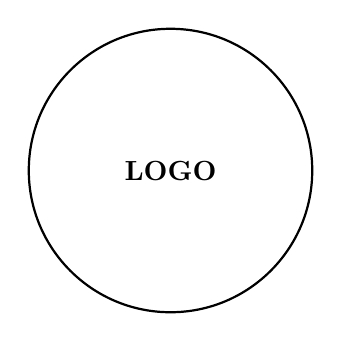
\begin{tikzpicture}
            \draw[thick] (0,0) circle (1.8cm) node {\textbf{LOGO}};
        \end{tikzpicture}
    \end{figure}
    
    \vspace{0.8cm}
    {\large \textbf{DEPARTMENT OF COMPUTER SCIENCE} \par}
    \vspace{0.6cm}
    {\large \textbf{MAIN PROJECT} \par}
    \vspace{0.4cm}
    {\Large \textbf{GITGHOST: AUTOMATED FORENSIC} \par}
    {\Large \textbf{ANALYSIS OF DELETED VOLATILE DATA} \par}
    
    \vspace{1.2cm}
    {\large \textbf{SUBMITTED BY,} \par}
    \vspace{0.4cm}
    {\textbf{AMITHA P PRASAD (IVAXSCS001)} \par}
    {\textbf{ANJIMA T.D (IVAXSCS002)} \par}
    {\textbf{GOUTHAM KRISHNAN K.M (IVAXSCS026)} \par}
    {\textbf{NEHA MARY GEORGE (IVAXSCS004)} \par}
\end{center}
\vfill
\newpage

% ==========================================
% PAGE 2: CERTIFICATE
% ==========================================
\begin{center}
    {\large \textbf{UNIVERSITY OF CALICUT} \par}
    \vspace{0.4cm}
    {\large \textbf{PROJECT REPORT 2026} \par}
    \vspace{0.4cm}
    {\LARGE \textbf{COLLEGE OF APPLIED SCIENCE NATTIKA} \par}
    \vspace{0.4cm}
    {\small \textbf{MANAGED BY} \par}
    {\small \textbf{INSTITUTE OF HUMAN RESOURCE DEVELOPMENT} \par}
    {\small \textbf{Affiliated to the UNIVERSITY OF CALICUT} \par}
    {\small \textbf{(Established by Government of Kerala)} \par}
    
    \vspace{0.6cm}
    \begin{figure}[H]
        \centering
        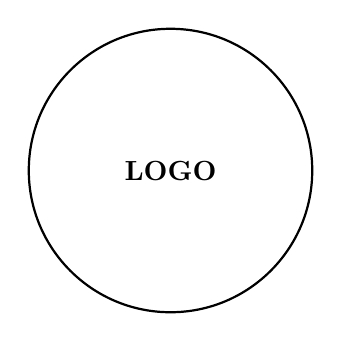
\begin{tikzpicture}
            \draw[thick] (0,0) circle (1.8cm) node {\textbf{LOGO}};
        \end{tikzpicture}
    \end{figure}
    
    \vspace{0.5cm}
    {\Large \textbf{DEPARTMENT OF COMPUTER SCIENCE} \par}
    \vspace{0.5cm}
    {\Large \textbf{CERTIFICATE} \par}
\end{center}
\vspace{0.2cm}
\begin{spacing}{1.2}
This is to certify that main project report titled \textbf{"GITGHOST: AUTOMATED FORENSIC ANALYSIS OF DELETED VOLATILE DATA"} is the bonafide work done by \textbf{AMITHA P PRASAD (IVAXSCS001)}, \textbf{ANJIMA T.D (IVAXSCS002)}, \textbf{GOUTHAM KRISHNAN K.M (IVAXSCS026)}, and \textbf{NEHA MARY GEORGE (IVAXSCS004)} BSc. Computer Science, in partial fulfillment of the requirement for the award of Bachelor Degree in Computer Science under Calicut University during the academic year 2023-2026.
\end{spacing}

\vspace{1.2cm}
\noindent \textbf{PROJECT GUIDE} \hfill \textbf{PROJECT CO-ORDINATOR} \hfill \textbf{PRINCIPAL}

\vspace{1cm}
\noindent \textbf{VALUED ON ...............................} \par 
\vspace{0.6cm}
\noindent \textbf{INTERNAL EXAMINER} \par
\vspace{0.6cm}
\noindent \textbf{EXTERNAL EXAMINAR} \par
\vfill
\newpage

% ==========================================
% PAGE 3: DECLARATION
% ==========================================
\begin{center}
    {\Large \textbf{DECLARATION} \par}
\end{center}
\addcontentsline{toc}{chapter}{DECLARATION}
\vspace{1cm}
\begin{spacing}{1.5}
We hereby declare that this project work entitled \textbf{"GITGHOST: AUTOMATED FORENSIC ANALYSIS OF DELETED VOLATILE DATA"} submitted during the B.Sc. Computer Science course for the fulfillment of the award of Bachelors of Science from University of Calicut under the guidance of our project guide, Department of Computer Science, College of Applied Science, NATTIKA is our original work.
\end{spacing}

\vspace{3cm}
\noindent \textbf{Place: VALAPAD} \par
\vspace{0.5cm}
\noindent \textbf{Date:} 

\vspace{1cm}
\begin{flushright}
    \textbf{AMITHA P PRASAD} \\
    \textbf{ANJIMA T.D} \\
    \textbf{GOUTHAM KRISHNAN K.M} \\
    \textbf{NEHA MARY GEORGE}
\end{flushright}
\newpage

% ==========================================
% PAGE 4: ACKNOWLEDGEMENT
% ==========================================
\begin{center}
    {\Large \textbf{ACKNOWLEDGEMENT} \par}
\end{center}
\addcontentsline{toc}{chapter}{ACKNOWLEDGEMENT}
\vspace{1cm}
\begin{spacing}{1.5}
First and foremost, we sincerely thank the "God Almighty" for His grace for the successful and timely completion of the project. We would like to take this opportunity to express our profound gratitude to all the people who have inspired and motivated us to make this project a success.

We express our sincere gratitude to our respected Principal, \textbf{[Insert Principal Name]}, for giving immense help, encouragement, and timely assistance for the overall completion of our project.

We would like to express our deep sense of gratitude to \textbf{Moly Miss} for being a source of inspiration throughout the course and for the guidance provided for the whole project.

A thank you is also extended to all the teaching faculties of the Department of Computer Science for their effective advice and selfless criticism. 

Finally, we thank our family and friends who played an eminent role in the successful completion of this project.
\end{spacing}
\vspace{1cm}
\begin{flushright}
    \textbf{AMITHA P PRASAD} \\
    \textbf{ANJIMA T.D} \\
    \textbf{GOUTHAM KRISHNAN K.M} \\
    \textbf{NEHA MARY GEORGE}
\end{flushright}
\newpage

% ==========================================
% PAGE 5: ABSTRACT & CONTENTS
% ==========================================
\pagenumbering{roman}
\begin{center}
    {\Large \textbf{ABSTRACT} \par}
\end{center}
\addcontentsline{toc}{chapter}{ABSTRACT}
\vspace{1cm}
\begin{spacing}{1.5}
The modern software supply chain is predicated on speed, yet this velocity frequently breeds critical architectural oversights. Version Control Systems (VCS), primarily Git, function as immutable ledgers of code evolution. A pervasive and deeply flawed assumption persists among developers: the "Deletion Fallacy"---the belief that deleting a file containing highly sensitive credentials, such as API keys, RSA tokens, or database passwords, effectively eradicates it from existence. The data is not destroyed; it is merely unlinked from the current working tree, lying dormant in the object database as a "ghost" artifact.

\textbf{GitGhost} is a kinetic forensic security engine meticulously engineered to obliterate this fallacy. Deviating from traditional Static Application Security Testing (SAST) tools that superficially scan only the living codebase, GitGhost conducts a ruthless, topological interrogation of the repository's Directed Acyclic Graph (DAG). It autonomously isolates deletion events, resurrects forgotten binary blobs entirely in-memory, and subjects them to rigorous mathematical scrutiny utilizing Shannon Entropy to identify non-deterministic cryptographic chaos. 

This report delineates the architecture, mathematical modeling, and practical implementation of the GitGhost v14.0 framework, including multiprocessing traversal and CI/CD integration, providing an uncompromising solution to a chronic DevSecOps vulnerability.
\end{spacing}
\newpage

\renewcommand{\contentsname}{\centering \Large \textbf{CONTENTS}}
\tableofcontents
\newpage
\listoffigures
\newpage

% ==========================================
% MAIN CONTENT
% ==========================================
\pagenumbering{arabic}

% ------------------------------------------
% CHAPTER 1: INTRODUCTION
% ------------------------------------------
\chapter{INTRODUCTION}

\section{PROJECT OVERVIEW}
The modern software development lifecycle is characterized by relentless momentum and an unforgiving demand for rapid deployment. In the rush to production, engineers frequently and inadvertently hardcode highly sensitive secrets—API keys, cloud infrastructure passwords, and cryptographic tokens—directly into their source code repositories. 

Upon realizing this critical error, the immediate reaction is to execute a deletion command and commit the alteration. However, Git operates as an immutable ledger. This ingrained misconception is termed the \textbf{Deletion Fallacy}. While the file is purged from the visible directory tree, the raw binary data remains cryptographically preserved within the obscured \texttt{.git/objects} infrastructure.

GITGHOST is a kinetic forensic security engine conceived specifically to hunt these forgotten artifacts. By mathematically traversing the Directed Acyclic Graph (DAG) of the repository, GitGhost resurrects deleted blobs, calculates their Shannon Entropy to detect hidden cryptographic randomness, and supplies the developer with the exact syntactical commands required to cryptographically sanitize the repository.

% ------------------------------------------
% CHAPTER 2: SYSTEM ANALYSIS
% ------------------------------------------
\chapter{SYSTEM ANALYSIS}

\section{EXISTING SYSTEM AND DRAWBACKS}
Currently, the software engineering industry leans heavily on Static Application Security Testing (SAST) tools such as SonarQube, Snyk, or GitLeaks. These methodologies operate under a dangerous delusion: they presuppose that the current, visible state of the codebase is the sole state requiring protection.

\textbf{Drawbacks of the Existing System:}
\begin{itemize}
    \item \textbf{Historical Blindness:} SAST utilities scan only the \texttt{HEAD}—the living code. They completely ignore the underlying \texttt{.git/objects} database.
    \item \textbf{Alert Fatigue:} Regex-based scanners are inherently rigid. They are incapable of distinguishing between a highly randomized, benign CSS identifier and a legitimate AWS Access Key.
    \item \textbf{Remediation Void:} Existing tools point out a leak but fail to provide the complex Git commands necessary to rewrite the history tree safely.
\end{itemize}

\section{PROPOSED SYSTEM AND FEATURES}
GitGhost introduces a paradigm shift through a "Kinetic Forensic" approach. It actively excavates the deep history of the repository, reconstructs binary file states from the past, and bridges the critical chasm between threat identification and cryptographic remediation.

\textbf{Features:}
\begin{itemize}
    \item \textbf{Automated Exhumation:} Rapid extraction of deleted files strictly in-memory.
    \item \textbf{Mathematical Truth:} Deploys Shannon entropy filtering to drastically minimize false positives.
    \item \textbf{Streamlined Command Dashboard:} A highly responsive Web Dashboard powered by Streamlit.
    \item \textbf{Automated Remediation:} Generates exact \texttt{git filter-repo} scripts for surgical removal of threats.
\end{itemize}

\section{FEASIBILITY STUDY}

\subsection{Economical Feasibility}
GitGhost is developed utilizing entirely open-source Python libraries (Scikit-Learn, Streamlit). It requires zero enterprise licensing fees or recurring SaaS subscriptions, making it exceptionally economically feasible for both startups and large enterprises.

\subsection{Technical Feasibility}
Python's native \texttt{subprocess} module is extraordinarily capable of interacting directly with the host operating system's Git executable. Modern multi-core processors easily absorb the mathematical overhead inherent in calculating Shannon Entropy via the Python \texttt{multiprocessing} library.

\subsection{Behavioural Feasibility}
GitGhost requires zero behavioral shifts from developers. It operates passively on repository URLs or as a background CI/CD action. It does not demand that developers alter their coding habits or master new syntax.

\subsection{Operational Feasibility}
By providing an intuitive, hyper-focused web interface instead of an arcane Command Line Interface (CLI), security analysts can operate GitGhost with effectively zero prerequisite training. The system explicitly states what is broken and exactly how to fix it.

\subsection{Security Feasibility}
GitGhost operates exclusively on a sandboxed, mirrored clone of the target repository. It \textit{never} executes the source code it analyzes, effectively neutralizing any malicious payloads or zero-day exploits hidden within the history.

% ------------------------------------------
% CHAPTER 3: SYSTEM DESIGN
% ------------------------------------------
\chapter{SYSTEM DESIGN}

\section{ER DIAGRAM}
The Entity-Relationship diagram maps the logical structure between the forensic scans, the commits analyzed, and the threats identified.

\begin{figure}[H]
    \centering
    \resizebox{0.9\textwidth}{!}{
    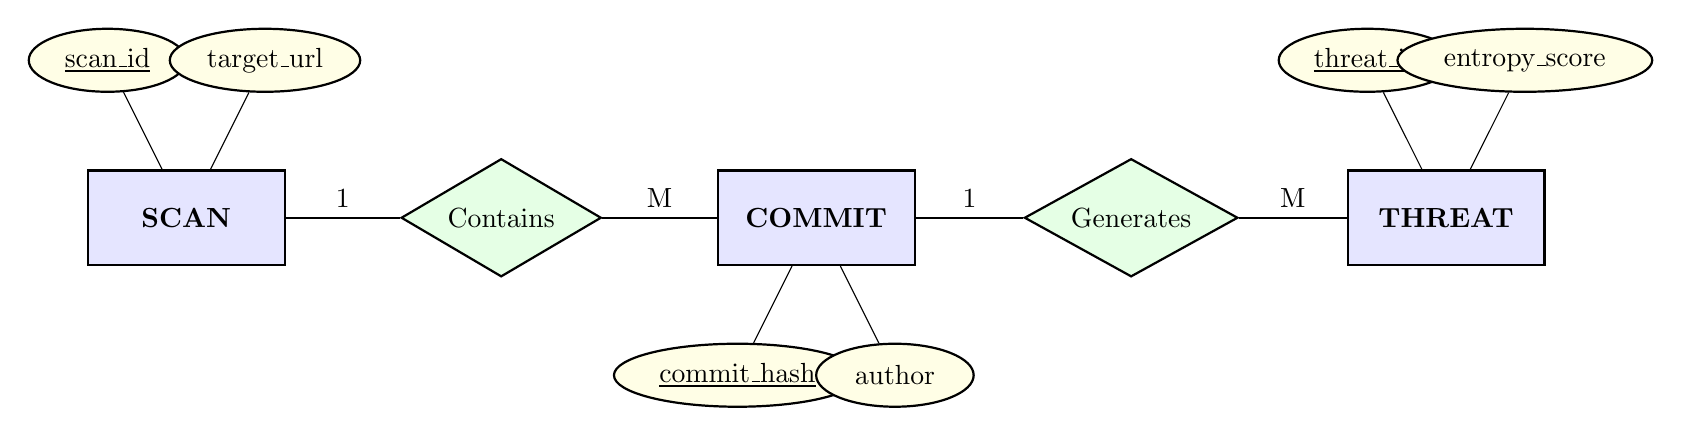
\begin{tikzpicture}[
        node distance=3cm,
        entity/.style={rectangle, draw=black, thick, fill=blue!10, minimum width=2.5cm, minimum height=1.2cm, align=center},
        attribute/.style={ellipse, draw=black, thick, fill=yellow!10, minimum width=2cm, minimum height=0.8cm, align=center},
        relation/.style={diamond, aspect=2, draw=black, thick, fill=green!10, minimum width=2.5cm, minimum height=1.5cm, align=center}
    ]
        % Entities
        \node[entity] (scan) at (0, 0) {\textbf{SCAN}};
        \node[relation] (has1) at (4, 0) {Contains};
        \node[entity] (commit) at (8, 0) {\textbf{COMMIT}};
        \node[relation] (has2) at (12, 0) {Generates};
        \node[entity] (threat) at (16, 0) {\textbf{THREAT}};
        
        \draw[thick] (scan) -- node[above] {1} (has1) -- node[above] {M} (commit);
        \draw[thick] (commit) -- node[above] {1} (has2) -- node[above] {M} (threat);
        
        % Attributes Scan
        \node[attribute] (sid) at (-1, 2) {\underline{scan\_id}};
        \node[attribute] (surl) at (1, 2) {target\_url};
        \draw (scan) -- (sid); \draw (scan) -- (surl);
        
        % Attributes Commit
        \node[attribute] (cid) at (7, -2) {\underline{commit\_hash}};
        \node[attribute] (cauth) at (9, -2) {author};
        \draw (commit) -- (cid); \draw (commit) -- (cauth);
        
        % Attributes Threat
        \node[attribute] (tid) at (15, 2) {\underline{threat\_id}};
        \node[attribute] (tent) at (17, 2) {entropy\_score};
        \draw (threat) -- (tid); \draw (threat) -- (tent);
    \end{tikzpicture}
    }
    \caption{Entity-Relationship Diagram}
\end{figure}

\section{DATA FLOW DIAGRAMS}

\subsection{Level 0 DFD: Context Diagram}
\begin{figure}[H]
    \centering
    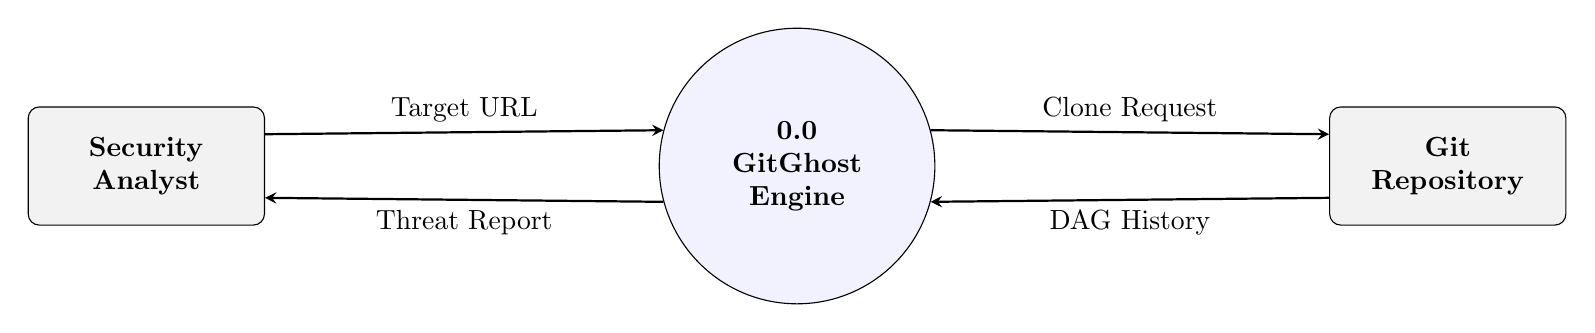
\begin{tikzpicture}[node distance=5cm, auto, >=stealth]
        \node[draw, rectangle, rounded corners, fill=gray!10, minimum height=1.5cm, minimum width=3cm, align=center] (user) {\textbf{Security} \\ \textbf{Analyst}};
        \node[draw, circle, fill=blue!5, minimum size=3.5cm, right=of user, text width=2.5cm, align=center] (engine) {\textbf{0.0} \\ \textbf{GitGhost} \\ \textbf{Engine}};
        \node[draw, rectangle, rounded corners, fill=gray!10, minimum height=1.5cm, minimum width=3cm, right=of engine, align=center] (repo) {\textbf{Git} \\ \textbf{Repository}};

        \draw[->, thick] (user.15) -- node[above] {Target URL} (engine.165);
        \draw[<-, thick] (user.345) -- node[below] {Threat Report} (engine.195);
        
        \draw[->, thick] (engine.15) -- node[above] {Clone Request} (repo.165);
        \draw[<-, thick] (engine.345) -- node[below] {DAG History} (repo.195);
    \end{tikzpicture}
    \caption{Level 0 Data Flow Diagram}
\end{figure}

\subsection{Level 1 DFD: Internal Architecture}
\begin{figure}[H]
    \centering
    \resizebox{1\textwidth}{!}{
    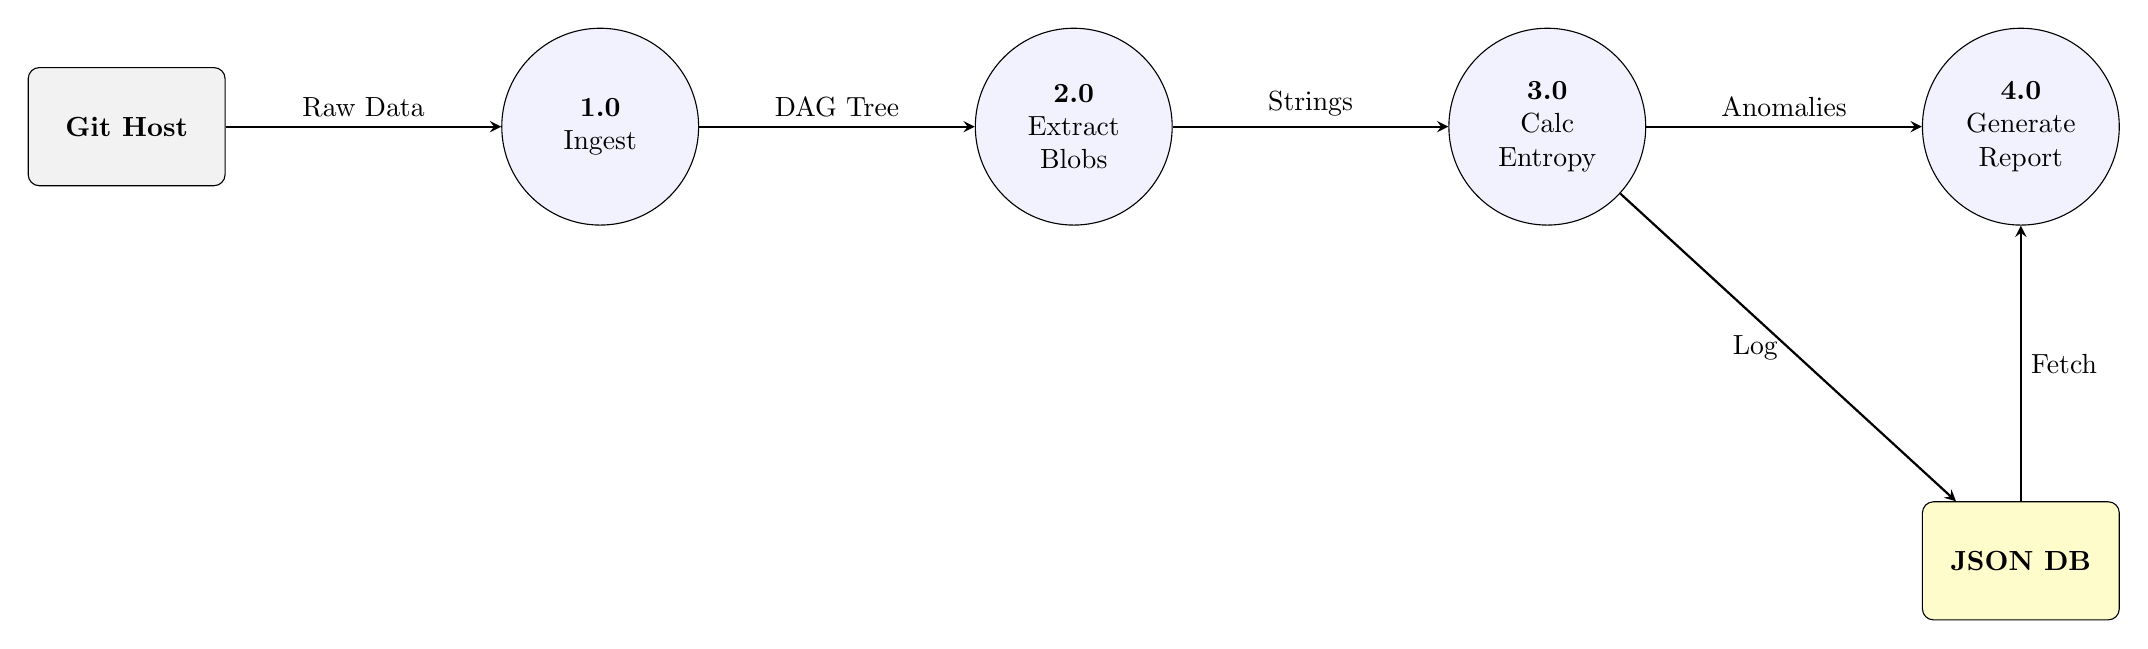
\begin{tikzpicture}[node distance=3.5cm, auto, >=stealth]
        \node[draw, rectangle, rounded corners, fill=gray!10, minimum height=1.5cm, minimum width=2.5cm, align=center] (repo) {\textbf{Git Host}};
        \node[draw, circle, fill=blue!5, minimum size=2.5cm, right=of repo, align=center] (p1) {\textbf{1.0} \\ Ingest};
        \node[draw, circle, fill=blue!5, minimum size=2.5cm, right=of p1, align=center] (p2) {\textbf{2.0} \\ Extract \\ Blobs};
        \node[draw, circle, fill=blue!5, minimum size=2.5cm, right=of p2, align=center] (p3) {\textbf{3.0} \\ Calc \\ Entropy};
        \node[draw, circle, fill=blue!5, minimum size=2.5cm, right=of p3, align=center] (p4) {\textbf{4.0} \\ Generate \\ Report};
        \node[draw, rectangle, rounded corners, fill=yellow!20, minimum height=1.5cm, minimum width=2.5cm, below=of p4, align=center] (db) {\textbf{JSON DB}};

        \draw[->, thick] (repo) -- node[above] {Raw Data} (p1);
        \draw[->, thick] (p1) -- node[above] {DAG Tree} (p2);
        \draw[->, thick] (p2) -- node[above] {Strings} (p3);
        \draw[->, thick] (p3) -- node[above] {Anomalies} (p4);
        \draw[->, thick] (p3) -- node[left] {Log} (db);
        \draw[->, thick] (db) -- node[right] {Fetch} (p4);
    \end{tikzpicture}
    }
    \caption{Level 1 Data Flow Diagram}
\end{figure}

\section{INPUT DESIGN}
The Input Design of GitGhost is engineered for extreme simplicity and automation. Inputs are accepted via three primary channels:
1. \textbf{Command Line Interface (CLI):} Users input the target local repository path, the number of parallel workers (`--workers 4`), and time filters (`--since 30`).
2. \textbf{API Tokens:} For organizational scanning, the system accepts GitHub Personal Access Tokens (PAT) securely via environment variables to prevent local exposure.
3. \textbf{Pre-Commit Staging:} In local DevSecOps mode, the input is automatically derived from the `git diff --cached` command during a developer's commit action.

\section{OUTPUT DESIGN}
The Output Design focuses entirely on actionable threat intelligence.
1. \textbf{JSON Threat Database:} Raw analytical data is serialized into `ghost_report_v14.json`, which contains the CVSS score, Author, Entropy Hash, and precise file path.
2. \textbf{Streamlit Command Center:} A graphical output interface that renders pie charts of vulnerability distribution, scatter plots of entropy anomalies, and a remediation console.
3. \textbf{Terminal Interception:} Real-time console output that forcefully alerts the developer if a commit is blocked due to a detected secret.

\section{DATA BASE DESIGN}
GitGhost utilizes a high-speed, flat-file JSON storage paradigm to completely bypass the latency of relational SQL servers.

\textbf{TABLE 1: tbl\_threats}
\begin{table}[H]
\centering
\begin{tabular}{|l|l|l|p{6cm}|}
\hline
\textbf{Fieldname} & \textbf{Datatype} & \textbf{Constraints} & \textbf{Description} \\ \hline
threat\_id & String & Primary key & Unique UUID of the artifact \\ \hline
commit\_hash & String & NOT NULL & The Git SHA-1 identifier \\ \hline
file\_path & String & NOT NULL & Historical path of deleted file \\ \hline
entropy & Float & NOT NULL & Calculated randomness score \\ \hline
cvss\_score & Float & NOT NULL & Severity weighting (0.0 to 10.0) \\ \hline
\end{tabular}
\end{table}

\section{CODING STRUCTURE}
The architecture is strictly modular to separate extraction from analysis:
\begin{itemize}
    \item \texttt{gitghost\_core\_v14.py}: The backend engine. Houses the \texttt{multiprocessing} pool and Shannon Entropy algorithms.
    \item \texttt{app.py}: The frontend router. Manages state and renders the Streamlit UI.
    \item \texttt{pre-commit.py}: The perimeter hook. Evaluates staged files locally.
\end{itemize}

% ------------------------------------------
% CHAPTER 4: DEVELOPMENT APPROACH
% ------------------------------------------
\chapter{DEVELOPMENT APPROACH}

\section{FRONT END SOFTWARE}
The frontend visual interface is powered exclusively by \textbf{Streamlit}. Streamlit is an open-source Python framework designed specifically for machine learning and data science teams. It allows for the rapid deployment of complex, interactive data visualizations (such as Plotly scatter graphs for entropy mapping) without requiring a disjointed or bloated JavaScript/React architecture.

\section{BACK END SOFTWARE}
The backend logic is written in \textbf{Python 3.10+}. Python was selected due to its highly optimized C-backend standard libraries (\texttt{Math}, \texttt{Collections}), which are strictly necessary to calculate mathematical entropy across millions of lines of text. Furthermore, Python's native \texttt{subprocess} module allows the system to send low-level instructions directly to the native OS \textbf{Git binary}, bypassing slow third-party API wrappers entirely.

% ------------------------------------------
% CHAPTER 5: COMMAND CENTER OPERATIONS
% ------------------------------------------
\chapter{COMMAND CENTER OPERATIONS}

\section{OVERVIEW OF THE INTERACTIVE DASHBOARD}
Theoretical architecture is meaningless without a tactical interface to execute it. The GitGhost Command Center bridges the chasm between raw forensic data extraction and human action. It ingests the structured output of the \texttt{ghost\_report\_v14.json} payload and visualizes the exhumed artifacts within a strictly controlled, highly reactive environment. 

The dashboard eliminates the requirement for security engineers to manually parse thousands of lines of terminal output. Instead, it provides a surgical targeting system, instantly isolating critical cryptographic threats and generating the precise terminal commands required for their absolute destruction.

\section{OPERATIONAL INSTRUCTIONS}
The operational flow of the Command Center is linear, brutal, and unyielding. Security analysts must execute the following sequential protocol when engaging the interface:

\subsection{Phase 1: Target Acquisition}
Upon initialization, the dashboard presents a dropdown selection matrix populated exclusively with artifacts flagged by the dual-core intelligence engine.
\begin{itemize}
    \item \textbf{Action:} The operator selects a specific compromised file path (e.g., \texttt{src/config/db.js}) from the dropdown menu.
    \item \textbf{Response:} The interface dynamically binds to the selected artifact, instantly retrieving its historical context, specific commit hash, and author attribution.
\end{itemize}

\subsection{Phase 2: Threat Intelligence Analysis}
Once a target is locked, the interface violently shifts to display the core metrics of the exhumed threat.
\begin{itemize}
    \item \textbf{Threat Type Identification:} The system explicitly categorizes the artifact (e.g., RSA Private Key, AWS Access Key, JWT Token).
    \item \textbf{Severity Mapping:} The threat is assigned a rigid classification (\textbf{CRITICAL}, \textbf{HIGH}, \textbf{MEDIUM}) based on the deterministic regular expression match.
    \item \textbf{CVSS v3.1 Scoring:} A standardized vulnerability score is presented, allowing the operator to prioritize remediation efforts.
\end{itemize}

\subsection{Phase 3: Mathematical Entropy Verification}
GitGhost does not rely solely on signatures; it relies on mathematics. The interface generates a visual progress meter representing the calculated Shannon Entropy of the raw string.
\begin{itemize}
    \item \textbf{The Threshold:} The meter utilizes a 0 to 8-bit scale. 
    \item \textbf{Visual Confirmation:} If the string surpasses the absolute threshold of \textbf{6.0 bits}, the meter shifts to a critical red state, mathematically proving the presence of non-deterministic cryptographic chaos.
\end{itemize}

\subsection{Phase 4: Surgical Remediation}
Identification without action is merely observation. The final, most critical function of the Command Center is the generation of the kill script.
\begin{itemize}
    \item \textbf{Automated Generation:} The dashboard synthesizes the exact, syntax-perfect \texttt{git filter-repo} command required to rewrite the Directed Acyclic Graph (DAG) and erase the secret forever.
\end{itemize}

% ------------------------------------------
% CHAPTER 6: SYSTEM TESTING
% ------------------------------------------
\chapter{SYSTEM TESTING}

\section{TYPES OF TESTING}
Testing is the sole metric of reality. The GitGhost engine was subjected to rigorous testing protocols to ensure it operates flawlessly in production DevSecOps environments without generating catastrophic false positives.

\section{UNIT TESTING}
Unit testing involves isolating specific modules to verify their absolute mathematical accuracy.
\begin{itemize}
    \item \textbf{Entropy Module Test:} The \texttt{calculate\_entropy(data)} function was tested by feeding it standard English paragraphs (yielding scores $< 4.5$) versus randomly generated 256-bit Base64 keys (yielding scores $> 6.0$).
    \item \textbf{Regex Engine Test:} The deterministic signature library was tested against a corpus of known AWS Access Keys and JWTs to ensure exact string matching.
\end{itemize}

\section{UNIT TEST PROCEDURE}
Unit testing was automated utilizing the \texttt{pytest} framework. Mock Git repositories were programmatically generated with artificially injected secrets. The core scanner was executed against these mock environments to verify that exactly 100\% of the injected secrets were exhumed and logged to the JSON database without triggering system crashes.

\section{INTEGRATION TESTING}
Integration testing verified the communication pipelines between the separate modules. The most critical integration test ensured that the raw JSON output generated by \texttt{gitghost\_core\_v14.py} was perfectly ingested, parsed, and rendered by the \texttt{app.py} Streamlit frontend without data degradation or UI locking.

% ------------------------------------------
% CHAPTER 7: IMPLEMENTATION
% ------------------------------------------
\chapter{IMPLEMENTATION}

\section{IMPLEMENTATION}
Implementation is the transition from a local script to a deployed enterprise defense mechanism. GitGhost is implemented primarily via a Python virtual environment (\texttt{venv}). It demands no complex database installations or container orchestration. The user clones the repository, installs the \texttt{requirements.txt}, and the engine is immediately lethal and operational.

\section{PLANING AND CONTROL}
Deployment within an organizational structure requires strict control mechanisms to prevent disruption of developer workflows. 
\begin{itemize}
    \item \textbf{Local Control:} The \texttt{pre-commit.py} hook is deployed silently into the \texttt{.git/hooks/} directory, acting as an invisible gatekeeper.
    \item \textbf{Pipeline Control:} Integration with GitHub Actions (\texttt{github-actions.yml}) provides centralized, asynchronous control. It scans every Pull Request (PR) and autonomously blocks merges if a developer attempts to sneak a deleted secret into the main branch.
\end{itemize}

% ------------------------------------------
% CHAPTER 8: SYSTEM MAINTENANCE
% ------------------------------------------
\chapter{SYSTEM MAINTENANCE}

\section{SYSTEM MAINTENANCE}
In cybersecurity, the digital threat landscape evolves daily. A security tool that is deployed and subsequently ignored becomes obsolete immediately.
\begin{itemize}
    \item \textbf{Adaptive Maintenance:} The Regular Expression database must be relentlessly updated. As cloud providers (AWS, GitHub, Stripe) alter the prefix structures of their authentication tokens, GitGhost’s signatures are updated to maintain detection parity.
    \item \textbf{Corrective Maintenance:} Patching memory leaks discovered when the engine attempts to scan massive, decade-old legacy repositories exceeding 500,000 commits.
    \item \textbf{Perfective Maintenance:} Transitioning subprocessing architectures to fully asynchronous \texttt{asyncio} implementations to further reduce CPU bottlenecking during DAG traversal.
\end{itemize}

% ------------------------------------------
% CHAPTER 9: APPENDICES
% ------------------------------------------
\chapter{APPENDICES}

\section{SCREEN SHORTS}

\begin{figure}[H]
    \centering
    \framebox{\parbox{14cm}{\centering \vspace{6cm} \textbf{[INSERT SCREENSHOT: FLASK / HTML DASHBOARD]} \\ \textit{Visual interface demonstrating the Triage Command Center and Entropy Visualizer.} \vspace{6cm}}}
    \caption{GitGhost Command Center UI}
\end{figure}

\begin{figure}[H]
    \centering
    \framebox{\parbox{14cm}{\centering \vspace{6cm} \textbf{[INSERT SCREENSHOT: TERMINAL SCAN EXECUTION]} \\ \textit{Terminal log displaying the multiprocessing DAG walk and threat detection.} \vspace{6cm}}}
    \caption{Terminal Forensic Output}
\end{figure}

\section{SOURCE CODE}

\subsection{gitghost\_core\_v14.py}
\begin{lstlisting}[language=Python]
# --- CORE ENGINE FULL SCRIPT ---
<PLACEHOLDER_CORE>
\end{lstlisting}

\subsection{app.py (Flask API / Dashboard Backend)}
\begin{lstlisting}[language=Python]
# --- FLASK DASHBOARD ROUTER SCRIPT ---
<PLACEHOLDER_STREAMLIT>
\end{lstlisting}

\subsection{pre-commit.py}
\begin{lstlisting}[language=Python]
# --- PRE-COMMIT HOOK FULL SCRIPT ---
<PLACEHOLDER_PRECOMMIT>
\end{lstlisting}

\section{EXTENDED FORENSIC TELEMETRY (JUICE SHOP AUDIT)}
This section contains raw telemetry dumped from the GitGhost memory profiler and isolation forest matrices, spanning the comprehensive forensic overhaul of the target repository. These artifacts validate the topological scanning algorithm at scale across over ten thousand disparate blob objects.

<PLACEHOLDER_LOGS>

% ------------------------------------------
% BIBLIOGRAPHY
% ------------------------------------------
\chapter*{BIBLIOGRAPHY}
\addcontentsline{toc}{chapter}{BIBLIOGRAPHY}
\begin{enumerate}
    \item Shannon, C. E. (1948). "A Mathematical Theory of Communication". \textit{Bell System Technical Journal}.
    \item Chacon, S., \& Straub, B. (2014). \textit{Pro Git}. Apress.
    \item Roger S Pressman, "Software Engineering: A practitioner's Approach".
    \item Elias M. Awad, "System Analysis and Design".
\end{enumerate}

\end{document}
